\chapter{Machine Learning Methods}

NOTE: Good way to start is with the question: What is a model? We can discuss the differences between mechanistic models (i.e. physics equations), their free parameters (constants of nature) and other types of models such as the non-parametric, nonlinear models used in machine learning. Further, we can discuss how machine learning models often display have the desirable trait of being a \textbf{universal approximator}. This will naturally lead to a discussion of function expansions (Taylor, Fourier, other polynomial expansions, etc...) and how they scale poorly (exponential) with increasing dimension. Machine learning models essentially allow us to do the same thing: perform a function expansion given data but in a way that can scale well to arbitrary dimension (features) of data. This allows us to build predictive models without necessarily needing to prescribe *all* of the physics. From another perspective, this framework allows us to incorporate our physics knowledge from well-behaved or linearized domains in order to *fit the residual* behavior with a sophisticated data-driven approach.

discuss role in science in particular (i.e. calibration, modeling, etc...)

discuss pushback against use in science and need for methods which simultaneously provide uncertainty bounds. Also describe types of ML e.g. supervised, unsupervised, generative, etc...

this is a good place for the Chihuahua vs Muffin meme... and use this to motivate incorportating physical knowledge into the machine learning process as a key feature for scientific applications... we have more constraints!

also discuss statistical v.s. deep learning


%------------------------------------------------------------------------------------------%

\section{Exploratory Data Analysis}
\subsection{Correlation}
\subsection{Mutual Information}


%------------------------------------------------------------------------------------------%

\section{Model Training Methodology}
\subsection{Data Sampling}
Dr. Lary's method (from Gaussian Process Code) for representative sampling to reduce data size
\begin{itemize}
\item Testing holdout set
\item k-fold Cross Validation
\end{itemize}
We should use this subsection to discuss why k-fold cross validation is ideal where data size/time permits so that you can get a sense of each model's dependence on the input data. Similarly, it is important we end the discussion by pointing out that the final \textbf{production} model is to be trained on the \textit{entire} dataset after we have evaluated which model is best to use and the ideal hyperparameters, etc...
\subsection{Model Evaluation}
Here we should discuss how we evaluate models, e.g. scatter plots, quantile-quantile plots, histograms, confusion matrices, various correctness metrics, etc...
\subsection{Hyperaprameter Selection}
Discuss grid search vs random search vs Bayesian Optimization, etc...
\subsection{Occam's Razor and Feature Importance Ranking}
I should point out my contributions to various julia packages in MLJ for doing feature importance determination here
\subsubsection{Linear Regression}
\subsubsection{Tree Based Methods}
\subsubsection{Neural Networks}
Perhaps explore ideas from Chris Olah's blog??? From a perspective of basic function composition... as in Rackauckas's blog
\subsubsection{Shapley Values}
Here we can discuss Shapley Values as a model agnostic method for feature importance rankings with the caveat that their computation can take quite a while...


%------------------------------------------------------------------------------------------%

\section{Supervised Regression Techniques}
\subsection{Neural Networks}
\subsection{Gaussian Process Regression}

Based on my notes from \href{https://github.com/john-waczak/MLJGaussianProcesses.jl/blob/main/notebooks/gpr/gaussian_process_regression_overview.ipynb}{this repo}

The following is based on the book \textbf{Gaussian Processes for Machine Learning} by Carl Edward Rasmussen and Christopher K. I. Williams \cite{gaussian-process-book}. You can find the free online book \href{https://gaussianprocess.org/gpml/}{here}.

To explain/derive the Gaussian Process model for regression, let's first consider a motivating example: \textbf{Linear Regression}. We will use this guiding example to derive GRP from a \textit{weight space view}. After this derivation, we will suggest a simpler, but more abstract derivation using a \textit{function space view}. First let's set up some data we can use for training:

\subsubsection{The Weight Space View}

We consider a dataset $\mathcal{D}$ with $n$ observations
\begin{equation}
  \mathcal{D} = \Big\{ (\mathbf{x}_i, y_i) \;\Big\vert \; i = 1,...,n\Big\}
\end{equation}

\begin{itemize}[noitemsep, nolistsep]
\item $\mathbf{x}_i$ is the $i^{th}$ D-dimensional input (feature) vector
\item $y_i$ is the $i^{th}$ target
\end{itemize}

Linear regression is easily understood in terms of \textit{linear algebra}. We therefore collect our dataset $\mathcal{D}$ into a $D \times n$ dimensional \href{https://en.wikipedia.org/wiki/Design_matrix}{\textbf{Design Matrix}}. Note that we have used a transposed definition (features are rows, records are columns) as Julia is a column-major language (like Matlab and Fortran).

\begin{equation}
  X := \begin{pmatrix}
    \vdots & \vdots & & \vdots \\
    \mathbf{x}_1 & \mathbf{x}_2 & ... & \mathbf{x}_n \\
    \vdots & \vdots & & \vdots
  \end{pmatrix}
\end{equation}

and our targets into a target vector

\begin{equation}
  \mathbf{y} := (y_1, ..., y_n)
\end{equation}

so that the full training set becomes

\begin{equation}
  \mathcal{D} := (X, \mathbf{y})
\end{equation}

Standard linear regression is a model of the form
\begin{equation}
  f(\mathbf{x}) = \mathbf{x}^T\mathbf{w}
\end{equation}

where $\mathbf{w}$ is the $D$-dimensional vector of weights. By minimizing the mean-squared-error between our model and targets, one can show that the optimal weights are given by

\begin{equation}
  \mathbf{w} = (XX^T)^{-1}X\mathbf{y}
\end{equation}


Note, this can also be easily obtained geometrically by finding the vector with the shortest distance to the hyperplane defined by the column space of $X$. This corresponds to solving the \href{https://en.wikipedia.org/wiki/Ordinary_least_squares#Normal_equations}{normal equations}.

\begin{equation}
  XX^T \mathbf{w} = X\mathbf{y}
\end{equation}

The following demonstrates this procedure on a simple dataset

\begin{figure}[h]
  \begin{centering}
    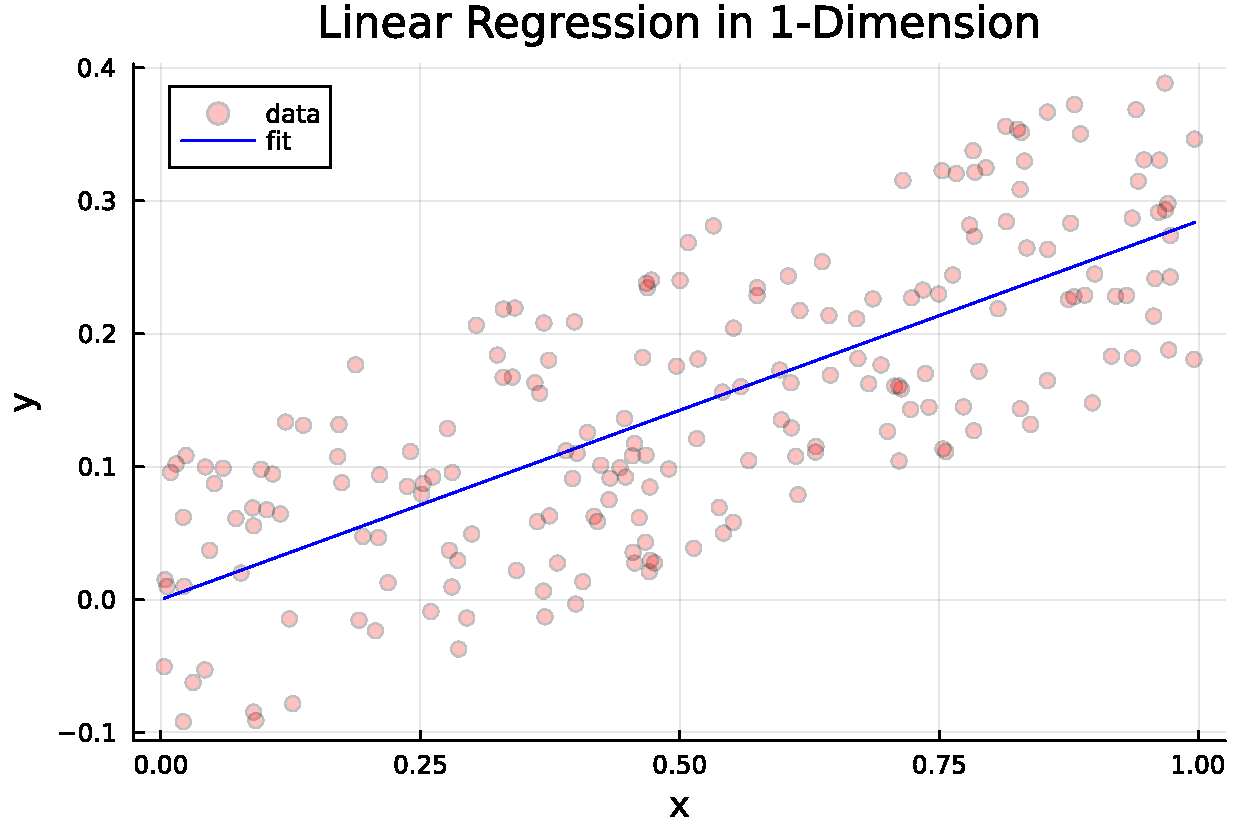
\includegraphics[width=0.9\columnwidth]{ml-figures/gpr/linear-regression.pdf}
  \end{centering}
  \caption{A standard linear regression fit on some noisy data.}
\end{figure}

We can also fit a y-intercept (aka \textit{bias}) by augmenting the design matrix $X$ to contain an extra row with all $1$'s, i.e.

\begin{equation}
  X[D+1, :] = (1, ..., 1)
\end{equation}

Standard linear regression assumes that are data $\mathcal{D}$ are perfect but we can clearly see that the above data are noisy. To account for this, we need to make our model \textit{Bayesian} by augmenting it to consider the measurement error. We define
\begin{align}
    f(\mathbf{x}) &= \mathbf{x}^T\mathbf{w} \\
    \mathbf{y} &= f(\mathbf{x}) + \mathbf{\epsilon} \\
    \mathbf{\epsilon} &\sim \mathcal{N}(0, \sigma_n^2)
\end{align}

or, in words, our observed values differ from the \textit{truth} by identically, independently, distributed Gaussian noise with mean $0$ and variance $\sigma_n^2$. The assumption that the noise is i.i.d. is critical because it allows us to simplify the \textit{likelihood} function by separating out each individual contribution by our datapoints:

\begin{align}
    p(\mathbf{y}\vert X,\mathbf{w}) &:= \prod\limits_i^n p(\mathbf{y}_i \vert \mathbf{x}_i, \mathbf{w}) \\
    &= \prod\limits_i^n \frac{1}{\sqrt{2\pi\sigma_n^2}}\exp\left( -\dfrac{(\mathbf{y}_i-\mathbf{x}_i^T\mathbf{w})^2}{2\sigma_n^2}\right)\\
    &= \dfrac{1}{(2\pi\sigma_n^2)^{n/2}}\exp\left( -\frac{1}{2\sigma_n^2}\lvert \mathbf{y} - X^T\mathbf{w}\rvert^2 \right) \\
    &= \mathcal{N}\left(X^T\mathbf{w}, \sigma_n^2I\right)
\end{align}

To perform inference with this updated model, we apply Baye's Rule, that is:


\begin{equation}
  p(\mathbf{w}\vert \mathbf{y}, X) = \dfrac{p(\mathbf{y}\vert X, \mathbf{w})p(\mathbf{w})}{p(\mathbf{y}\vert X)}
\end{equation}
where
\begin{itemize}[noitemsep, nolistsep]
\item $p(\mathbf{w}\vert \mathbf{y}, X)$ is the \textit{posterior distribution}
\item $p(\mathbf{y}\vert X, \mathbf{w})$ is the \textit{likelihood}
\item $p(\mathbf{w})$ is the \textit{prior distribution}
\item $p(\mathbf{y} \vert X)$ is the \textit{marginal likelihood}, i.e. the normalization constant
\end{itemize}
It is now that the utility of choosing gaussian distributions for our likelihood and prior becomes clear. We have
\begin{align}
  p(\mathbf{w}\vert\mathbf{y},X) &\propto \exp\left(-\frac{1}{2\sigma_n^2}(\mathbf{y}-X^T\mathbf{w})^T(\mathbf{y}-X^T\mathbf{w}) \right)\exp\left(-\frac{1}{2}\mathbf{w}^T\Sigma_p^{-1}\mathbf{w}\right)
\end{align}
Taking the log and expanding leads to
\begin{align}
  \log(p(\mathbf{w}\vert \mathbf{y}, X))&= \frac{1}{2}\left[ \frac{1}{\sigma_n^2}\mathbf{y}^T\mathbf{y} - \frac{1}{\sigma_n^2}\mathbf{y}^TX^T\mathbf{w} - \frac{1}{\sigma_n^2}\mathbf{w}^TX\mathbf{y} + \frac{1}{\sigma_n^2}\mathbf{w}^TXX^T\mathbf{w} + \mathbf{w}^T\Sigma_p^{-1}\mathbf{w}\right] \\
  &= \frac{1}{2}\left[ \mathbf{w}^T\left(\frac{1}{\sigma_n^2}XX^T+\Sigma_p^{-1}\right)\mathbf{w} -\left(\frac{1}{\sigma_n^2}\mathbf{y}^TX^T\right)\mathbf{w} - \mathbf{w}^T\left(\frac{1}{\sigma_n^2}X\mathbf{y}\right)  + \mathbf{y}^T\frac{1}{\sigma_n^2}\mathbf{y}\right]\\
  &= \mathbf{w}^TA\mathbf{w} - B^T\mathbf{w} - \mathbf{w}^TB + C
\end{align}
where we have defined
\begin{align}
    A &:= \frac{1}{\sigma_n^2}XX^T + \Sigma_p^{-1} \\
    B &:= \frac{1}{\sigma_n^2}X\mathbf{y} \\
    C &:= \mathbf{y}^T\frac{1}{\sigma_n^2}\mathbf{y}
\end{align}
Now we can complete the square so that
\begin{equation}
    \mathbf{w}^TA\mathbf{w} - B^T\mathbf{w} - \mathbf{w}^TB + C = \left(\mathbf{w} - \bar{\mathbf{w}} \right)^TA\left(\mathbf{w} - \bar{\mathbf{w}} \right) + K
    \end{equation}
    leading to 
    \begin{align}
    \bar{\mathbf{w}} &= A^{-1}B = \frac{1}{\sigma_n^2}\left(\frac{1}{\sigma_n^2}XX^T + \Sigma_p^{-1}\right)^{-1}X\mathbf{y} \\
    K &= C- \bar{\mathbf{w}}^TA\bar{\mathbf{w}}
\end{align}
Since $K$ does not depend on $\mathbf{w}$ directly, it may be absorbed into the normalization of $p(\mathbf{w}\vert \mathbf{y}, X)$. Thus we are left with
\begin{align}
    p(\mathbf{w}\vert\mathbf{y},X) &= \mathcal{N}\left( \bar{\mathbf{w}}=\frac{1}{\sigma_n^2}A^{-1}X\mathbf{y}, \Sigma=A^{-1}\right) \\
    A &= \frac{1}{\sigma_n^2}XX^T+\Sigma_p^{-1}
\end{align}
This result gives us the gaussian distriubtion over the space of possible parameter vectors $\mathbf{w}$. To use this distribution to make predictions, consider a newly supplied testpoint $\mathbf{x}_*$. We want to find
\begin{equation}
    p(y_* \vert \mathbf{x}_*, \mathbf{y}, X)
\end{equation}
We do this by marginalizing over our weight distribution, i.e.
\begin{equation}
    p(y_* \vert \mathbf{x}_*, \mathbf{y}, X) = \int_{\mathbf{w}} p(y_*\vert \mathbf{x}_*,\mathbf{w})p(\mathbf{w}\vert \mathbf{y}, X)d\mathbf{w}
\end{equation}
If we make the further assumption that testing points are i.i.d. guassian distriubted, we see that this integral is the product of two gaussians and therefore is also a guassian. To find the mean and covariance of the predictive distribution, we check
\begin{align} 
    \bar{y}_* &= \mathbb{E}[y_*] = \mathbb{E}[\mathbf{x}_*^T\mathbf{w}] = \mathbf{x}_*^T\mathbb{E}[\mathbf{w}] = \mathbf{x}_*^T\bar{\mathbf{w}} \\
    \text{Cov}(y_*) &= \mathbb{E}[(y_*-\bar{y}_*)(y_*-\bar{y}_*)^T] \\
    &= \mathbb{E}[(\mathbf{x}_*^T\mathbf{w}-\mathbf{x}_*^T\bar{\mathbf{w}})(\mathbf{x}_*^T\mathbf{w}-\mathbf{x}_*^T\bar{\mathbf{w}})^T] \\
    &= \mathbb{E}[\mathbf{x}_*^T(\mathbf{w}-\bar{\mathbf{w}})(\mathbf{w}-\bar{\mathbf{w}})^T\mathbf{x}_*] \\
    &= \mathbf{x}_*^T\mathbb{E}[(\mathbf{w}-\bar{\mathbf{w}})(\mathbf{w}-\bar{\mathbf{w}})^T]\mathbf{x}_* \\
    &= \mathbf{x}_*^T\text{Cov}(\mathbf{w})\mathbf{x}_* \\
    &= \mathbf{x}_*^TA^{-1}\mathbf{x}_*
\end{align}
so that
\begin{equation}
    \boxed{p(y_* \vert \mathbf{x}_*, \mathbf{y}, X) = \mathcal{N}\left(\mathbf{x}_*^T\mathbf{w},\;  \mathbf{x}_*^TA^{-1}\mathbf{x}_*\right)}
\end{equation}


Let's now take a break from our Bayesian regression discussion and return to the standard linear regression model for a moment. The key drawback of linear models like this is, of course, that they're \textit{linear}!. Considering that many (most) \textit{interesting} relationships are non-linear, how can we extend our simple linear model to enable us to perform complicated non-linear fits?

In the parlance of machine learning, the simple solution is to do \href{https://en.wikipedia.org/wiki/Feature_engineering}{feature engineering}. If our inital feature vector is
\begin{equation}
    \mathbf{x} = (x_1, ..., x_n)
\end{equation}
we can use our \textit{expertise} to concoct new combinations of these features to produce the agumented vector
\begin{equation}
    \tilde{\mathbf{x}} = (x_1, ..., x_n, x_1^2, \;sin(x_2), \;x_5x_7/x_4,\;...)
\end{equation}

As an example, a linear classifier is unable to distinguish points inside a circle from those outside just from the $(x,y)$ coordinates alone. Augmenting the feature vector to include the squared radius $x^2+y^2$ as a new feature removes this obstacle. This works because the \textit{linear} part of linear regression only refers to the fact that our model takes \textit{linear combinations} of feature variables to produce it's output. There is no restriction that the features themselves need to be independent variables! This same idea is what makes methods like \href{https://www.pnas.org/doi/10.1073/pnas.1517384113}{SINDy} work which use libraries of polynomial combinations of base features.

Constructing new features is often more art than science. To standardize the process, let's abstract the mapping from the original feature vector $\mathbf{x}$ to the augmented vector $\tilde{\mathbf{x}}$. This is accomplished via the projection map $\phi:\mathbb{R}^D \to \mathbb{R}^N$ where
\begin{equation}
    \mathbf{x} \mapsto \tilde{\mathbf{x}} = \phi(\mathbf{x})
\end{equation}
The result is that our linear model updates to become
\begin{equation}
    f(\mathbf{x}) := \phi(\mathbf{x})^T\mathbf{w}
\end{equation}
where the weight vector has gone from $D$ dimensional to $N$ dimensional. Similarly, the normal equations for $\mathbf{w}$ update to become
\begin{equation}
    \mathbf{w} = (\Phi\Phi^T)^{-1}\Phi\mathbf{y}
\end{equation}
where $\Phi = \phi(X)$ is the $N\times n$ matrix resulting from applying $\phi$ columnwise to $X$.

The following example shows how to use such a mapping to produce a quadratic polynomial fit.

\begin{figure}[h]
  \begin{centering}
    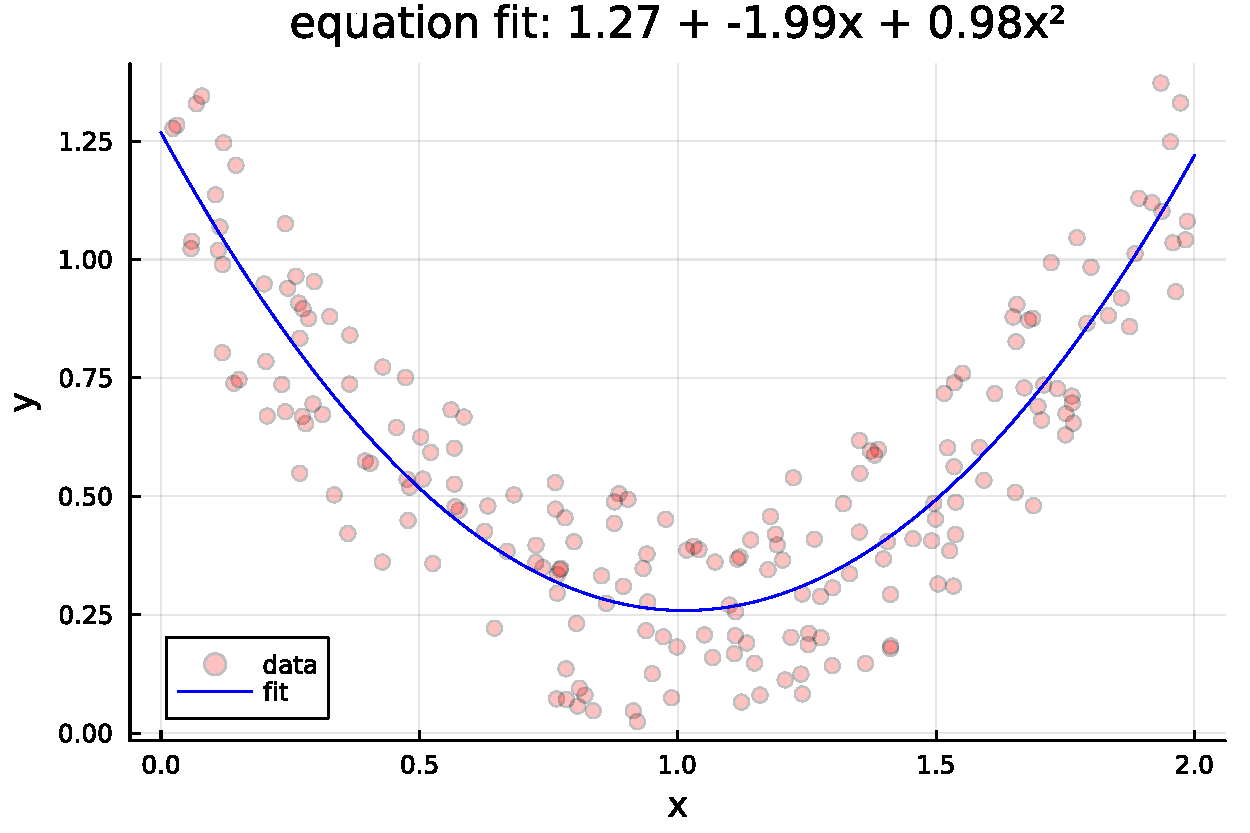
\includegraphics[width=0.85\columnwidth]{ml-figures/gpr/polynomial-regression.pdf}
  \end{centering}
  \caption{An example of polynomial regression for which we fit a quadratic polynomial to some noisy data.}
  \label{fig:polynomial-regression}
\end{figure}
We see from Figure \ref{fig:polynomial-regression} that our linear regression model found a great fit for a 2nd order polynomial when supplied with polynomial features. Let's update our Bayesian regression scheme to reflect the use of our feature projection map $\phi$. First we define
\begin{align}
  \Phi &:= \phi(X) \\
  \phi_* &:= \phi(\mathbf{x}_*)
\end{align}

Our predictive distribution therefore becomes
\begin{align}
  p(y_* \vert \mathbf{x}_*, X, \mathbf{y}) &= \mathcal{N}\left(\frac{1}{\sigma_n^2}\phi_*^TA^{-1}\Phi\mathbf{y}, \;\phi_*^TA^{-1}\phi_*\right) \\
  A &= \frac{1}{\sigma_n^2}\Phi\Phi^T + \Sigma_p^{-1}
\end{align}
Great! Now we can do our Bayesian inference with non-linear features given by $\phi$. There is a \textit{massive} problem with this approach, however. Our order 2 polynomial map $\phi$ takes us from a $D$ dimenional feature vector to $(D+1)!$ many. This means that as we add more features to our feature map, the dimension of the resulting vector will quickly become prohibitively large. Looking at our current model equations, we see that the bottleneck is the matrix inversion of $A$ which requires we invert an $N\times N$ matrix. Our prediction (i.e. the mean) involves multiplication on the right by the $n$ dimensional vector $\mathbf{y}$. With that in mind, perhaps we can reformulate the above into an equivalent form using at most an $n\times n$ dimensional matrix.

Let $K:= \Phi^T\Sigma_p\Phi$. Observe the following:
\begin{align}
  \frac{1}{\sigma_n^2}\Phi(K+\sigma_n^2I) &= \frac{1}{\sigma_n^2}\Phi\left(\Phi^T\Sigma_p\Phi + \sigma_n^2I \right) \\
  &= \frac{1}{\sigma_n^2}\Phi\Phi^T\Sigma_p\Phi + \Phi I \\
  &= \left(\frac{1}{\sigma_n^2}\Phi\Phi^T \right)\Sigma_p\Phi + \left(\Phi I \Phi^{-1}\Sigma_p^{-1} \right)\Sigma_p\Phi \\
  &= \left(\frac{1}{\sigma_n^2}\Phi\Phi^T + \Sigma_p^{-1}\right)\Sigma_p\Phi \\
  &= A\Sigma_p\Phi
\end{align}

From there we see that
\begin{align}
    A^{-1}\frac{1}{\sigma_n^2}\Phi\left(K+\sigma_n^2I\right) &= \Sigma_p\Phi \\
    \Rightarrow \frac{1}{\sigma_n^2}A^{-1}\Phi &= \Sigma_p\Phi\left(K + \sigma_n^2I\right)^{-1} \\
    \Rightarrow \frac{1}{\sigma_n^2}\phi_*^TA^{-1}\Phi &= \phi_*^T\Sigma_p\Phi\left(K + \sigma_n^2I\right)^{-1}
\end{align}
For the covariance, we utilize the matrix inversion lemma \textcolor{red}{(ADD REFERENCE HERE)} which states
\begin{equation}
    (Z + UWV^T)^{-1} = Z^{-1} - Z^{-1}U(W^{-1} + V^TZ^{-1}U)^{-1}V^TZ^{-1}
\end{equation}
With the identification
\begin{align}
    Z^{-1} &\to \Sigma_p \\
    W^{-1} &\to \sigma_n^2I \\
    V &\to \Phi \\
    U &\to \Phi
\end{align}
we find
\begin{align}
    \Sigma_p - \Sigma_p\Phi\left(\Sigma_p + \Phi^T\Sigma_p\Phi \right)^{-1}\Phi^T\Sigma_p  &= \left(\Sigma_p^{-1} + \Phi\frac{1}{\sigma_n^2}I\Phi^T\right)^{-1}\\
    &= \left(\frac{1}{\sigma_n^2}\Phi\Phi^T + \Sigma_p^{-1}\right)^{-1}  \\
    &= A^{-1}
\end{align}
Thus, we have the equivalent form for our predictive distribution:
\begin{equation}
    \boxed{p(y_*\vert \mathbf{x}_*, X, \mathbf{y}) =\\ \mathcal{N}\left( \phi_*^T\Sigma_p\Phi(K+\sigma_n^2I)^{-1}\mathbf{y}, \; \phi_*^T\Sigma_p\phi_* - \phi_*^T\Sigma_p\Phi(K+\sigma_n^2I)^{-1}\Phi^T\Sigma_p\phi_*\right)}
\end{equation}
where the pesky $N\times N$ term has been replaced by the $n\times n$ matrix $\Phi^T\Sigma_p\Phi$.


We now make the the \textit{key} observation that the only matrices that appear in the above expression are
\begin{align}
    &\Phi^T\Sigma_p\Phi, &\phi_*^T\Sigma_p\phi_* \\
    &\phi_*^T\Sigma_p\Phi, &\Phi^T\Sigma_p\phi_*
\end{align}
whose matrix elements we can write abstractly as
\begin{equation}
    \phi(\mathbf{x})^T\Sigma_p\phi(\mathbf{x}')
\end{equation}

To fit our model, we must determine appropriate values for the symmetric, positive semi-definite covariance matrix $\Sigma_p$ (and $\sigma_n$ too, technically). Instead, we observe that this matrix product is a quadratic form which we can think of as representing an inner product on our transformed vectors:
\begin{equation}
    K_{ij} = k(\mathbf{x}_i, \mathbf{x}_j) = \langle \phi(\mathbf{x}_i), \phi(\mathbf{x}_j)\rangle
\end{equation}
We call the function $k(\mathbf{x},\mathbf{x}')$ the \textit{kernel function} or the \textit{covariance function}.

All we need to perform the above calculations are the matrix elements of K applied to our data $\mathcal{D}$ and any test points $\mathbf{x}_*$ we wish to apply our model to. In effect, this means we are free to use feature vectors \href{https://www.youtube.com/watch?v=XUj5JbQihlU&t=25m53s}{of any dimension, including $\infty$}. The idea here is that the kernel function represents an inner product over \textit{some} vector space. As it turns out, the RBF kernel corresponds to a an \href{https://math.stackexchange.com/questions/276707/why-does-a-radial-basis-function-kernel-imply-an-infinite-dimension-map}{infinite dimensional feature vector}.

There are many choices for the kernel function. One of the most popular is the RBF (radial basis function) kernel, also commonly referred to as the \textit{squared exponential kernel}:
\begin{equation}
    k_{\text{rbf}}(\mathbf{x}, \mathbf{x}') := \sigma_f^2\exp(-\frac{1}{2\ell^2}\lvert \mathbf{x}-\mathbf{x}'\rvert^2)
\end{equation}

where $\sigma_f^2$ is the *signal variance* and $\ell$ denotes the similarity length scale.

For notational convenience, let's define
\begin{align}
    K &:= k(X,X) \\
    K_{**} &:= k(X_*, X_*) \\
    K_{*} &:= k(X, X_*)
\end{align}

then, our predictive distribution takes the final, \textit{clean} form
\begin{equation}
    \boxed{p(\mathbf{y}_* \vert X_*, X, \mathbf{y}) = \mathcal{N}\left( K_*^T(K+\sigma_n^2I)^{-1}\mathbf{y},\; K_{**}-K_{*}^T(K+\sigma_n^2I)^{-1}K_*\right)}
\end{equation}
This is the \textit{end-result} of Gaussian Process Regression acheived via the \textit{weight-space view}.


\subsubsection{The Function-space View}

So far our approach has been to generalize the standard linear regression model to allow for fitting over a (possibly infinite) basis of features with consideration for measurement and model uncertainty (our Bayesian priors). In essence, the idea was to fit the distribution of all possible weights conditioned on the available training data, $p(\mathbf{w} \vert X, \mathbf{y})$. A second \textit{equivalent} approach is to instead consider the distribution of all possible model function $f(\mathbf{x})$. By constructing a Bayesian prior over this space, we constrain the space of possible model functions and learn a \textit{distribution} over all allowed model functions, $p(f \vert X, \mathbf{y})$. To do so we will need to develop the abstract machinery of distributions over function spaces. When these distributions are Gaussian, the result is called a \textbf{Gaussian process}.

By this point, we are very familiar with the Gaussian distribution, a.k.a. the Normal distribtion $\mathcal{N}(\mu, \sigma^2)$. This distribution is defined by a mean value $\mu$ and a variance $\sigma^2$. It's \textit{big brother} is the \textbf{Multivariate Normal Distribution}, $\mathcal{N}(\mathbf{\mu}, \Sigma)$, described be a vector of means $\mathbf{\mu}$ and a covariance matrix $\Sigma$. A natural question, then, is can we generalize the concept of the Gaussian distribution from $N$ dimensions to being defined over a continuous field? This leads us naturally to the development of a so-called \textbf{Gaussian Process}.\\

\fbox{
  \parbox{0.8\columnwidth}{
    \noindent\textbf{Definition}: A \textit{Gaussian Process}, $\mathcal{GP}$, is a collection of random variables for which any finite subset are described by a joint Gaussian distribution.
  }
}\\


To see where this comes from, recall that in our previous derivation, we already made the assumption that all our our data points $\mathcal{D}$ are i.i.d. Gaussian distributed. A gaussian process is the natural extension of this and makes the assumption that the continuous set from which are data are sampled are **so Guassian** that any finite sample will be jointly Gaussian distributed. The term *process* is used to distinguish between finite collections of random variables (distributions) and their continuous counterparts described here.

Because each finite subset of this continuous collection is jointly gaussian, we can completely specify a Gaussian Process with two functions: the mean function $m(\mathcal{x})$ and the covariance function $k(\mathbf{x},\mathbf{x}')$. To denote this, we typically write
\begin{equation}
    f(\mathbf{x}) \sim \mathcal{GP}(m(\mathbf{x}), k(\mathbf{x},\mathbf{x}'))
\end{equation}

To see this in action, recall our Bayesian regression model
\begin{equation}
  f(\mathbf{x} = \phi(\mathbf{x})^T\mathbf{w} \qquad \mathbf{w}\sim\mathcal{N}(\mathbf{0}, \Sigma_p)
\end{equation}
where we have set the prior on $\mathcal{w}$ to have zero mean. The mean function is given by the expectation value of our model:
\begin{equation}
  \mathbb{E}[f(\mathbf{x})] = \phi(\mathbf{x})^T\mathbb{E}[\mathbf{w}] = 0
\end{equation}
and the covariance function is given by
\begin{equation}
  \mathbb{E}[f(\mathbf{x})f(\mathbf{x'})] = \phi(\mathbf{x})^T\mathbb{E}[\mathbf{w}\mathbf{w}^T]\phi(\mathbf{x}') = \phi(\mathbf{x})^T\Sigma_p\phi(\mathbf{x}')
\end{equation}

To repeat the point, the key feature of Gaussian processes is that finite subsets are jointly Gaussian distributed. Thus we can we can split our data into the testpoints $\mathcal{D}=(X,\mathbf{y})$ and testpoints $X_*$ t and treat each collection as joint distributions with the following priors:
\begin{equation}
  \begin{bmatrix} \mathbf{f} \\ \mathbf{f}_* \end{bmatrix} \sim \mathcal{N}\left(\mathbf{0},\begin{bmatrix} K(X,X) & K(X,X_*) \\ K(X_*,X) & K(X_*,X_*) \end{bmatrix}\right)
\end{equation}
where $\mathbf{f}:= f(X)$ and $\mathbf{f}_* = f(X_*)$.

To obtain our predictive distribution, $p(\mathbf{f}_* \vert X_*, X, \mathbf{y})$, we \textit{condition the joint prior distribution} on the observations. To see how this works, consider a general joint gaussian distribution given by
\begin{equation}
\begin{bmatrix} x \\ y \end{bmatrix} \sim \mathcal{N}\left( \begin{bmatrix}\mu_x \\ \mu_y\end{bmatrix},\; \begin{bmatrix} \Sigma_{xx} & \Sigma_{xy} \\ \Sigma_{yx} & \Sigma_{yy} \end{bmatrix}\right)
\end{equation}

define the centered values $\tilde{x} := x-\mu_x$ and $\tilde{y} := x-\mu_y$. Define the intermediate variable
\begin{equation}
    z := \tilde{x} - A\tilde{y}
\end{equation}
Note that since we've subtracted out the mean we have $\mathbb{E}[\tilde{x}] = \mathbb{E}[\tilde{y}] = \mathbb{E}[z] = 0$. Let's now find $A$.
\begin{align}
    \mathbb{E}[z\tilde{y}^T] &= \mathbb{E}[(\tilde{x}-A\tilde{y})\tilde{y}^T] \\
    &= \mathbb{E}[\tilde{x}\tilde{y}^T - A\tilde{y}\tilde{y}] \\
    &= \mathbb{E}[\tilde{x}\tilde{y}^T] - \mathbb{E}[A\tilde{y}\tilde{y}^T] \\
    &= \Sigma_{xy} - A\mathbb{E}[\tilde{y}\tilde{y}^T] \\
    &= \Sigma_{xy} - A\Sigma_{yy}
\end{align}
Therefore if we choose $A$ so that $z$ and $\tilde{y}$ are independent and uncorrelated, then $\Sigma_{zy} = \mathbb{E}[z\tilde{y}^T] = 0$. Using this assumption, we find
\begin{equation}
    0 = \mathbb{E}[z\tilde{y}^T] = \Sigma_{xy}-A\Sigma_{yy} \\ \Rightarrow \boxed{A = \Sigma_{xy}\Sigma_{yy}^{-1}}
\end{equation}
If we now condition $\tilde{x}$ on $\tilde{y}$ (i.e. look at $\tilde{x}$ when $\tilde{y}$ is constant), we find
\begin{align}
    \mathbb{E}[\tilde{x}\vert\tilde{y}] &= A\tilde{y} + \mathbb{E}[z] \\
    &= A\tilde{y} + 0 \\
    &= \Sigma_{xy}\Sigma_{yy}^{-1} \\
\end{align}
By manipulating this expression, we can now derive $\mathbb{E}[x\vert y]$ as follows:
\begin{align}
    \mathbb{E}[x\vert\tilde{y}] &= \mathbb{E}[\tilde{x}\vert\tilde{y}] + \mu_x \\
    &= \mu_x + \Sigma_{xy}\Sigma_{yy}^{-1}\tilde{y} \\
\end{align}
\begin{equation}
\boxed{\mathbb{E}[x\vert y] = \mu_x + \Sigma_{xy}\Sigma_{yy}^{-1}(y-\mu_y)}
\end{equation}

Similarly for the covariance, we have
\begin{align}
    \text{Cov}(x \vert y) &= \text{Cov}(\tilde{x}+\mu_x \vert \tilde{y}) \\
    &= \text{Cov}(\tilde{x}+\mu_x \vert \tilde{y} + \mu_y) \\
    &= \text{Cov}(\tilde{x}\vert(\tilde{y}+\mu_y)) \\
    &= \text{Cov}(\tilde{x}\vert \tilde{y}) \\
    &= \text{Cov}((z+A\tilde{y})\vert\tilde{y}) \\
    &= \text{Cov}(z) + {A\text{Cov}(\tilde{y})} \\
    &= \text{Cov}(z) + 0 \\
    &= \mathbb{E}[zz^T] \\
    &= \mathbb{E}[(\tilde{x}-A\tilde{y})(\tilde{x}-A\tilde{y})^T]\\
    &= \mathbb{E}[\tilde{x}\tilde{x}^T - A\tilde{y}\tilde{x}^T -x(A\tilde{y})^T + A\tilde{y}\tilde{y}^TA^T] \\
    &= \Sigma_{xx} - A\Sigma_{yx} - \Sigma_{xy}A^T + A\Sigma_{yy}A^T \\
    &= \Sigma_{xx}-(\Sigma_{xy}\Sigma_{yy}^{-1})\Sigma_{yx} - \Sigma_{xy}(\Sigma_{yy}^{-1})^T\Sigma_{xy}^T + \Sigma_{xy}\Sigma_y^{-1}\Sigma_{y}(\Sigma_{y}^{-1})^T\Sigma_{xy}^T \\
    &= \Sigma_{xx} - \Sigma_{xy}\Sigma{yy}^{-1}\Sigma_{xy}^T - \Sigma_{xy}(\Sigma_{yy}^{-1})^T\Sigma_{xy}^T + \Sigma_{xy}(\Sigma_{yy}^{-1})^T\Sigma_{xy}^T \\
    &= \Sigma_{xx}-\Sigma_{xy}\left[\Sigma_{yy}^{-1} - (\Sigma_{yy}^{-1})^T + (\Sigma_{yy}^{-1})^T \right]\Sigma_{xy}^T \\
    &= \Sigma_{xx} - \Sigma_{xy}\Sigma_{yy}^{-1}\Sigma_{yx}
\end{align}

\begin{equation}
\boxed{\text{Cov}(x \vert y) = \Sigma_{xx} - \Sigma_{xy}\Sigma_{yy}^{-1}\Sigma_{yx}}
\end{equation}
Armed with this identity for joint Guassian distributions, we are ready to derive the predictive distribution for Gaussian Process Regression. We find:
\begin{equation}
  p(\mathbf{f}_* \vert X_*, X, \mathbf{y} = \mathcal{N}\left( K_*^TK^{-1}\mathbf{f},\; K_{**}-K_*^TK^{-1}K_*\right).
\end{equation}
To account for noisy observations, we can augment our correlation function to include a noise offset. The joint distrubtion then becomes:
\begin{equation}
  \begin{bmatrix} \mathbf{f} \\ \mathbf{f}_* \end{bmatrix} \sim \mathcal{N}\left(\mathbf{0},\begin{bmatrix} K(X,X)-\sigma_n^2I & K(X,X_*) \\ K(X_*,X) & K(X_*,X_*) \end{bmatrix}\right)
\end{equation}
which leads to the predictive distribution
\begin{equation}
  \boxed{p(\mathbf{f}_* \vert X_*, X, \mathbf{y}) = \mathcal{N}\left( K_*^T\left[K + \sigma_n^2 I\right]^{-1}\mathbf{f},\; K_{**}-K_*^T\left[K + \sigma_n^2 I\right]^{-1}K_*\right)}
\end{equation}


\subsubsection{Doing it in Julia}

To see how we can use this in practice, let's first construct some sample data which we seek to model as a Gaussian Process
\begin{figure}[h]
  \begin{centering}
    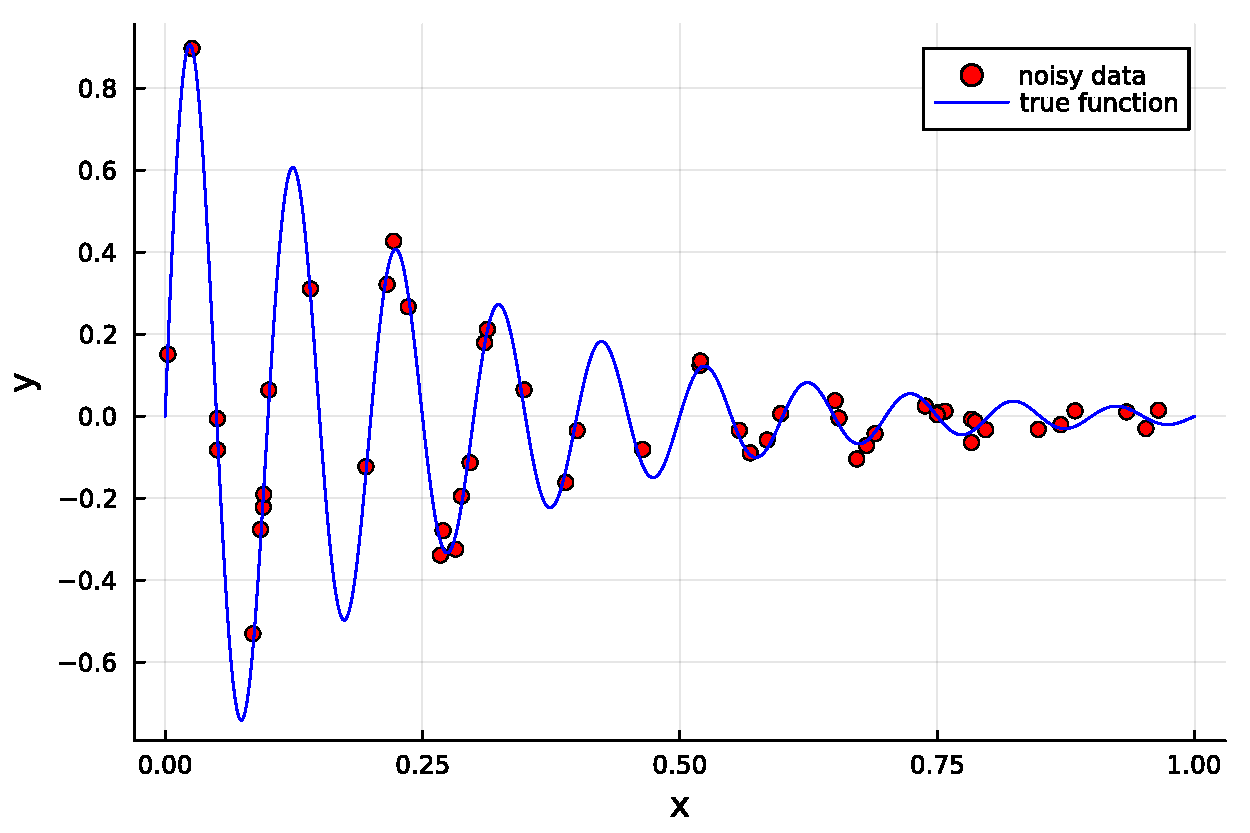
\includegraphics[width=0.8\columnwidth]{ml-figures/gpr/training-data.pdf}
  \end{centering}
\end{figure}

The excellent package \href{https://juliagaussianprocesses.github.io/KernelFunctions.jl/dev/userguide/}{KernelFunctions.jl} provides a clean interface to create various kernel functions and apply them to data to create our $K$-matrices. Due to the fact that kernel functions obey composition laws, we can easily build up complicated Kernels from basic pieces via function composition with $\circ$

\begin{figure}
  \centering
  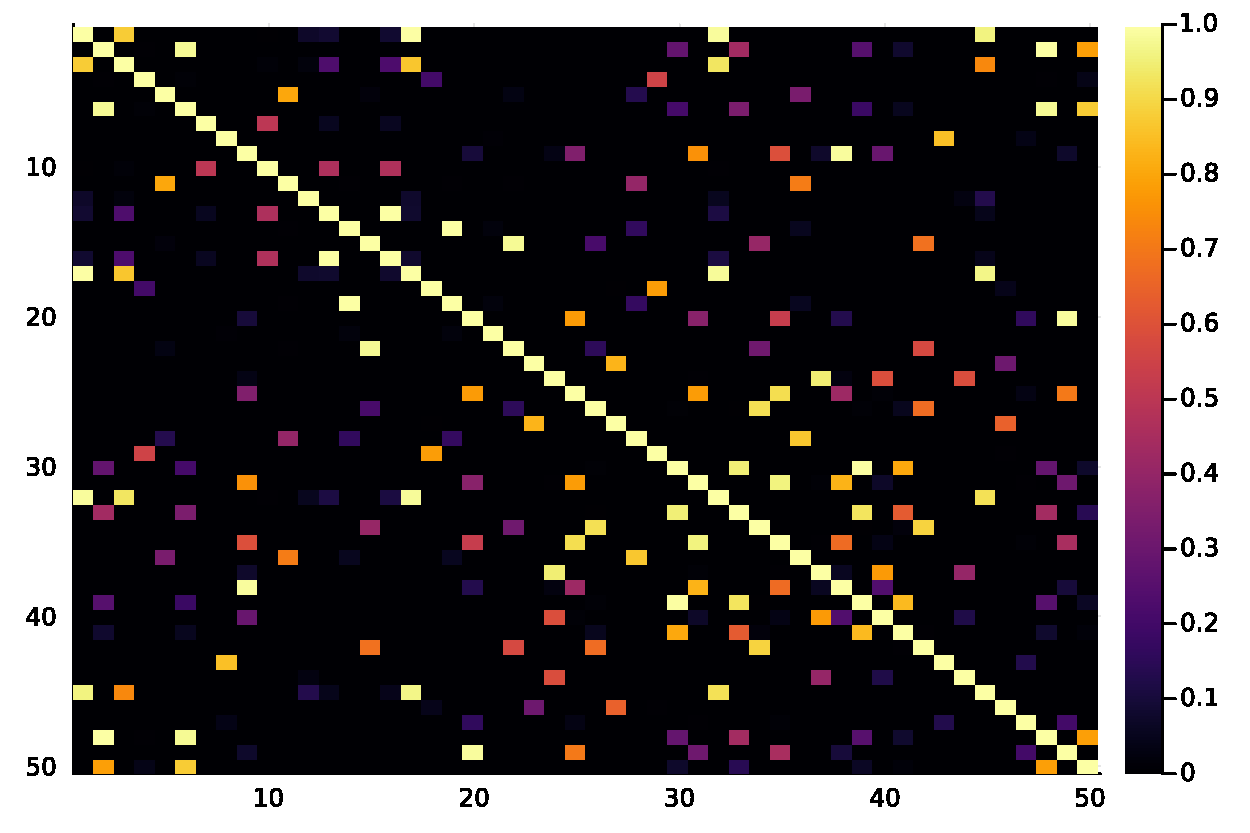
\includegraphics[width=0.8\columnwidth]{ml-figures/gpr/kernel-matrix.pdf}
\end{figure}
Unsurprisingly, there is a lot of activation on the diagonal as for a single datapoint $\mathbf{x}$, we have
\begin{equation}
    k(\mathbf{x},\mathbf{x}) = \exp\left(-\frac{0}{2\ell^2} \right) = 1.0
\end{equation}

The package \href{https://juliagaussianprocesses.github.io/AbstractGPs.jl/dev/}{AbstractGPs.jl} provides an excellent way to define Gaussian Processes by supplying mean and kernel functions. We can then sample from our GPs with a simple interface designed to extend the basic functions from \texttt{Statistics.jl}. From an \texttt{AbstractGP} we can construct a \texttt{FiniteGP} by \textit{indexing} into our datasets. The procedure can be summarized as follows
\begin{enumerate}
\item Build a kernel function $k(\cdot, \cdot)$ via composition using \texttt{KernelFunctions.jl}
\item Construct an a Gaussian Process $f\sim\mathcal{GP}$ abstractly using \texttt{AbstractGPs.jl}
\item Construct a finite representation of our GP, $f_x$, over our training data
\item Construct a posterior Gaussian Process from $f_x$ and our training targets $\mathbf{y}$.
\item Construct a finite representation of the posterior GP applied to our prediction data
\item Sample this final distribution to obatin a prediction via \texttt{mean()} and variances via \texttt{var()}. Alternatively, we can obtain a multivariate normal distribution for each point by calling \texttt{marginals()}.
\end{enumerate}

\begin{figure}[h]
  \centering
  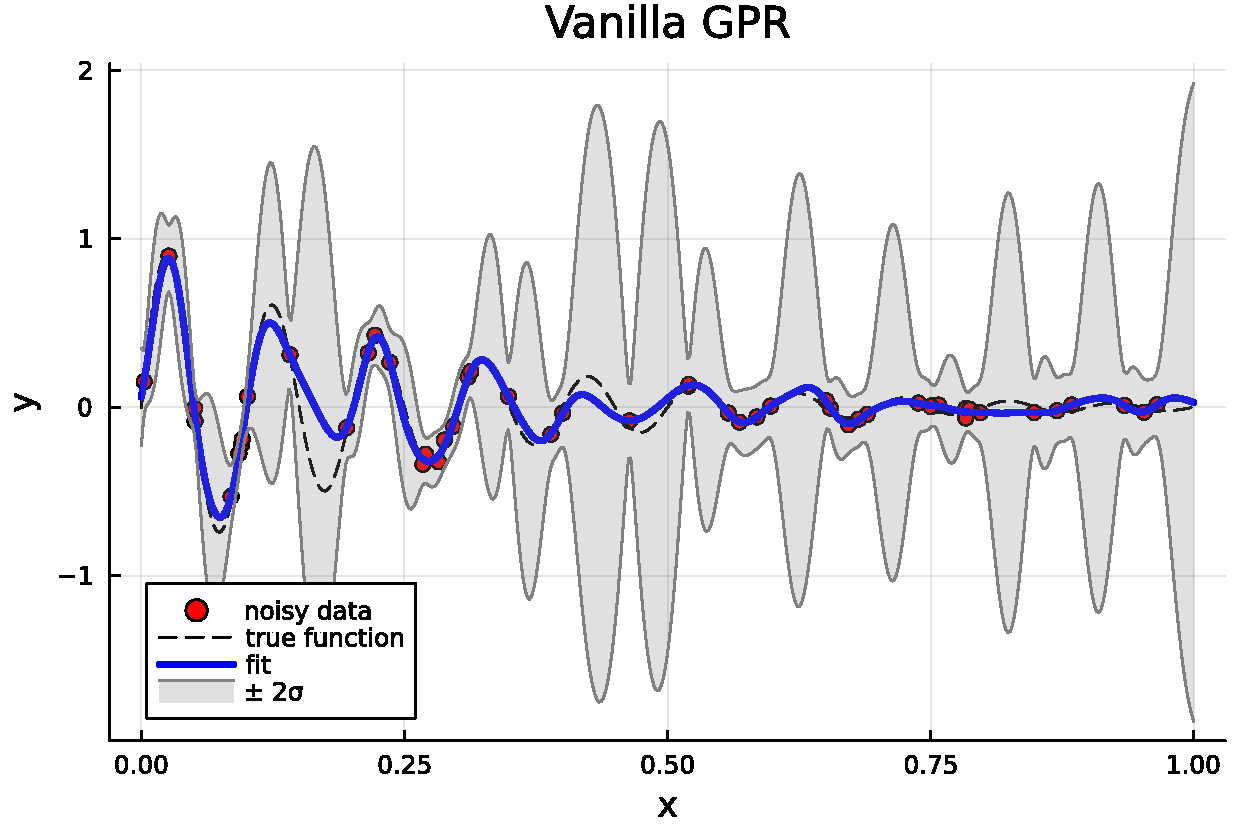
\includegraphics[width=0.85\columnwidth]{ml-figures/gpr/vanilla-gpr.pdf}
  \caption{A Gaussian Process fit to the training data illustrating the predication (means) and a $\pm 2\sigma$ uncertainty interval. We can clearly see how the uncertainty is larger for inputs far away from supplied training data.}
  \label{fig:vanilla-gpr}
\end{figure}

\subsubsection{Fitting the Kernel Hyperparameters}
At this point, it is easy to think we are finished; we \textit{already} fit the Guassian process. However, we were forced to choose values for both $\ell$ and $\sigma^2$ kernel parameters. How can we optimally select the ideal hyperparameters for our Gaussian Process? This question leads us into the realm of \href{https://gaussianprocess.org/gpml/chapters/RW5.pdf}{Bayesian Model Selection}. Rather than focusing specifically on our Gaussian Process model, let's take a step back and think about the process of model selection from a Bayesian perspective.

There are several levels of parameters in machine learning. At the lowest level, we have the model weights $\mathbf{w}$. Above that, we have model hyperparameters, $\theta$. At the top we have model structure $\mathcal{H}$. In our Bayesian framework, we can consider prior distributions defined at each of these levels which codify credences for how much we trust a particular model, hyperparameter, etc. At the bottom, we have
\begin{equation}
  p(\mathbf{w} \vert X, \mathbf{y}, \theta, \mathcal{H}_i) = \frac{p(\mathbf{y} \vert X, \mathbf{w}, \theta, \mathcal{H}_i) p(\mathbf{w}\vert \theta, \mathcal{H}_i) }{p(\mathbf{y}\vert X, \theta, \mathcal{H}_i)}
\end{equation}

If this looks confusing, consider Bayes rule for 3 events $R, H, S$. We have:
\begin{align}
  P(R \vert H, S) &= \frac{P(R,H,S)}{P(H,S)} \\
  &= \frac{P(H \vert R, S)P(R, S)}{P(H,S)}\\
  &= \frac{P(H \vert R, S)P(R\vert S)P(S)}{P(H\vert S)P(S)} \\
  &= \frac{P(H \vert R, S)P(R\vert S)}{P(H\vert S)}
\end{align}
To get the result, just think of $\theta$ and $\mathcal{H}_i$ as a single \textit{event} and translate the above to distribution functions. See \href{https://math.stackexchange.com/questions/1281454/bayes-rule-with-3-variables}{stack exchange link}.

The prior $p(\mathbf{w}\vert \theta, \mathcal{H}_i)$ encodes any knowledge we have about the parameters prior to seeing the data. The denominator is the \textit{marginal likelihood} and is given by
\begin{equation}
    p(\mathbf{y}\vert X, \theta, \mathcal{H}_i) = \int d\mathbf{w}\; p(\mathbf{y} \vert X, \mathbf{w}, \theta, \mathcal{H}_i)p(\mathbf{w}\vert \theta, \mathcal{H}_i)
\end{equation}
The next level up is to express the distribution of hyper-parameters $\theta$:
\begin{equation}
    p(\theta \vert X, \mathbf{y}, \mathcal{H}_i) = \frac{p(\mathbf{y}\vert X, \theta, \mathcal{H}_i)p(\theta \vert \mathcal{H}_i)}{p(\mathbf{y}\vert X, \mathcal{H}_i)}.
\end{equation}
Here $p(\theta \vert \mathcal{H}_i)$ is called the \textit{hyper-prior}. Similarly, the normalization constant is given by
\begin{equation}
    p(\mathbf{y}\vert X,\mathcal{H}_i) = \int d\theta \; p(\mathbf{y}\vert X, \theta, \mathcal{H}_i)p(\theta \vert \mathcal{H}_i).
\end{equation}
Finally, at the top level we have the set of possible model structures $\{\mathcal{H}_i\}$. This leads to
\begin{equation}
    p(\mathcal{H}_i \vert X, \mathbf{y}) = \frac{p(\mathbf{y} \vert X, \mathcal{H}_i)p(\mathcal{H}_i)}{p(\mathbf{y}\vert X)}
\end{equation}
with normlization constant
\begin{equation}
 p(\mathbf{y}\vert X) = \sum_i p(\mathbf{y} \vert X, \mathcal{H}_i)p(\mathcal{H}_i).
\end{equation}

Depending on the model details, these integrals may be intractable without approximations or Monte Carlo methods. Since we rarely have sufficient knowledge to form a hyperparameter prior, one often attempts to maximize the marginal likelihood $p(\mathbf{y} \vert X, \theta, \mathcal{H}_i)$ with respect to the hyperparameters $\theta$ instead. This is known as Type II Maximium Likelihood Estimation. \textcolor{red}{(Refer to prior section on this in the Theoretical Techniques chapter).} In the case of Gaussian Process Regression, we are once again saved by the fact that every piece has a convenient functional from resulting in analytically tractible integrals for the marginal likelihood function. We find
\begin{equation}
    \ln p(\mathbf{y}\vert X, \theta) = -\frac{1}{2}\mathbf{y}^T(K_f + \sigma_n^2 I)^{-1}\mathbf{y} - \frac{1}{2}\ln\lvert K_f + \sigma_n^2 I \rvert -\frac{n}{2}\ln(2\pi)
\end{equation}
where we have employed the natural logarithm remove the pesky exponentials and arrive at a very convenient form. Note that because the lograithm is monotonically increasing, the maximum of the log-marginal-likelihood will be the same as the marginal-likelihood itself. Provided this functional form, we can use our favorite optimization routine to obtain the kernel hyperparameters which maximize the likelihood of obtaining our data as illustrated in the following comparison figure.

\begin{figure}[h]
  \centering
  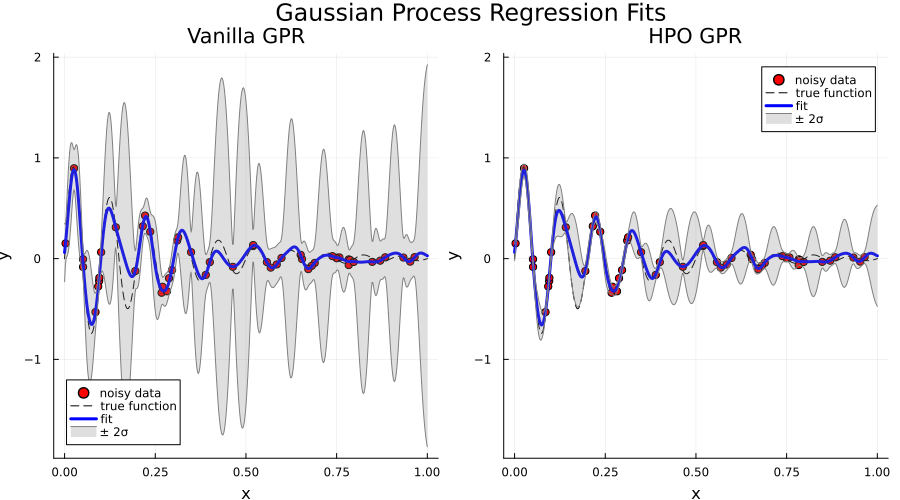
\includegraphics[width=0.85\columnwidth]{ml-figures/gpr/hpo-fit}
  \caption{Left: the original Gaussian Process obtained with our default choice of kernel parameters. Right: A much better Gaussian Process obtained after performing hyper-parameter optimization on the kernel parameters. Note how the mean function still does an excellent job fitting the data points while \textit{also} minimizing the uncertainty of the fit.}
  \label{fig:gpr-fit-comparison}
\end{figure}



\subsection{Decision Trees}


%------------------------------------------------------------------------------------------%

\section{Unsupervised Classification}
\subsection{k-Means Clustering}
\subsection{Self Organizing Maps}
\subsection{Generative Topographic Maps}


%------------------------------------------------------------------------------------------%

\section{Dimensionality Redution}
\subsection{PCA}
\subsection{ICA}
\subsection{t-SNE}


%------------------------------------------------------------------------------------------%

\section{Model Ensembling}
\subsection{Bagging}
e.g. Random Forests
\subsection{Boosting}
e.g. XGBoost
\subsection{Stacking}
e.g. Super Learners



%------------------------------------------------------------------------------------------%

\section{Uncertainty Quantification}
The focus of this section can be on the concept of uncertainty quantification. For many physics theories that are nicely linearized, uncertainty analysis can be easily accomplished at the level of first order sensitivites. That is, we can look at the Jacobian of our model to infer the behavior of small deviations about initial conditions. This approach does not easily extend to more complicated domains where the nonlinear effects dominate. Further, we also often want to establish ways to think about the fundamental instrument uncertainty for a measuring device. This can require meticulous calibrations which often assume a linear or polynomial fit... We can do better. Why not let the data tell us what the measurement uncertainty really is?

A good motivating example for the discussion of instrumental uncertainty is the use of a thermistor to measure temperature. One must assume a reasonable range of temperatures to establish the linear relationship between temperature and resistivity that is used determine the temperature. However, the material characteristics of the thermistor that introduce nonlinearities at extreme temperatures don't necessarily mean we should have to throw out measurements that do not fall within this well-behaved range. Rather, we can preform a more sophisticated *calibration* to learn a model mapping resistivity to temperature that can account for these effects.

This is the bread-and-butter of the MINTS sensing efforts. Often low-cost sensing solutions provide decent measurements within a limit domain. With quality data from superior (but often prohibitively expensive) reference instruments, we can improve the default calibration to improve the reliability of data (by reducing uncertainty) and extend it's domain of usefulness.

\subsection{Quantile Regression}
\subsection{Probabilistic Models}
e.g. discuss models like the GPR which fundamentally produce \textit{distributions}. Similarly for models like Neural Networks that can produce multiple outputs, we can train a model to predict both $\mu$ and $\sigma$ to make the model probabilistic.

\subsection{Conformal Prediction}



%------------------------------------------------------------------------------------------%

\section{Scientific Machine Learning}
\subsection{Physics-Informed Neural Networks}
\subsection{Universal Differential Equations}
\subsection{Adjoint Methods for ODEs: Neural Ordinary Differential Equations}
\subsection{Hamiltonian Neural Networks}



%------------------------------------------------------------------------------------------%

\section{Generative Methods}
\subsection{Auto Encoders}
\subsection{Generative Adversarial Networks}


%------------------------------------------------------------------------------------------%

\section{Data Assimilation}
\subsection{4d-Var}
\subsection{Kalman Filter}
\subsection{Extended Kalman Filter}
\subsection{continuous-discrete Extended Kalman Filter}


%------------------------------------------------------------------------------------------%

\section{Topological Data Analysis}
